\section{Evaluation}
\label{sec-evaluation}

%Metrics: what do you care about?
%Evaluation methodology: how did you evaluate?
%Results / discussions: if possible, provide intuitions and reasons for the
%result you got.

As described in the previous section, our study focuses on analyzing the AC and
DC power consumption ratios. Intuitively we would expect that DBI-AC and DBI-DC
help the AC and DC power consumption factors respectively. Table
\ref{table:dbi-ratios} illustrates the AC and DC ratio reductions for load and
store operations separately. The average ac/dc ratio improvements were computed
using the following formula:

$$ \TT{\% Improvement} = |\frac{\TT{DbiRatio} - \TT{nonDbiRatio}}{\TT{nonDbiRatio}}| \times 100\%$$

\begin{table}[!htb]
  \centering
    \begin{tabular}{| c | c |}
      \hline
      \textbf{DBI Ratio} & \textbf{\% Improvement} \\ \hline
     Load DC  & 68.59 \\ \hline
     Load AC  & 8.62  \\ \hline
     Store DC & 75.04 \\ \hline
     Store AC & 3.38  \\ \hline
    \end{tabular}
    \caption{Average AC/DC ratio reduction for load and store operations using
    DBI across all 28 MiBench applications}
    \label{table:dbi-ratios}
\end{table}

We can see the DBI-DC reduces the DC factor by 68.6 \% and 75.0 \% for load and
store operations whereas DBI-AC has a smaller reduction of 8.6 \%
and 3.4 \% respectively. Since the DC factor optimized the data values to
reduce the number of binary $0$'s \cite{low-power-dram}, we can conclude that
the values on cache misses for both load and store operations were
predominantly $0$'s  in the MiBench suite. This suggests that DBI, especially
DBI-DC does indeed improve the AC and DC power consumption ratios for
unencrypted memory systems. Next we compare DBI's impact on unencrypted versus
encrypted memory systems.

\begin{figure}[!htb]
  \centering
  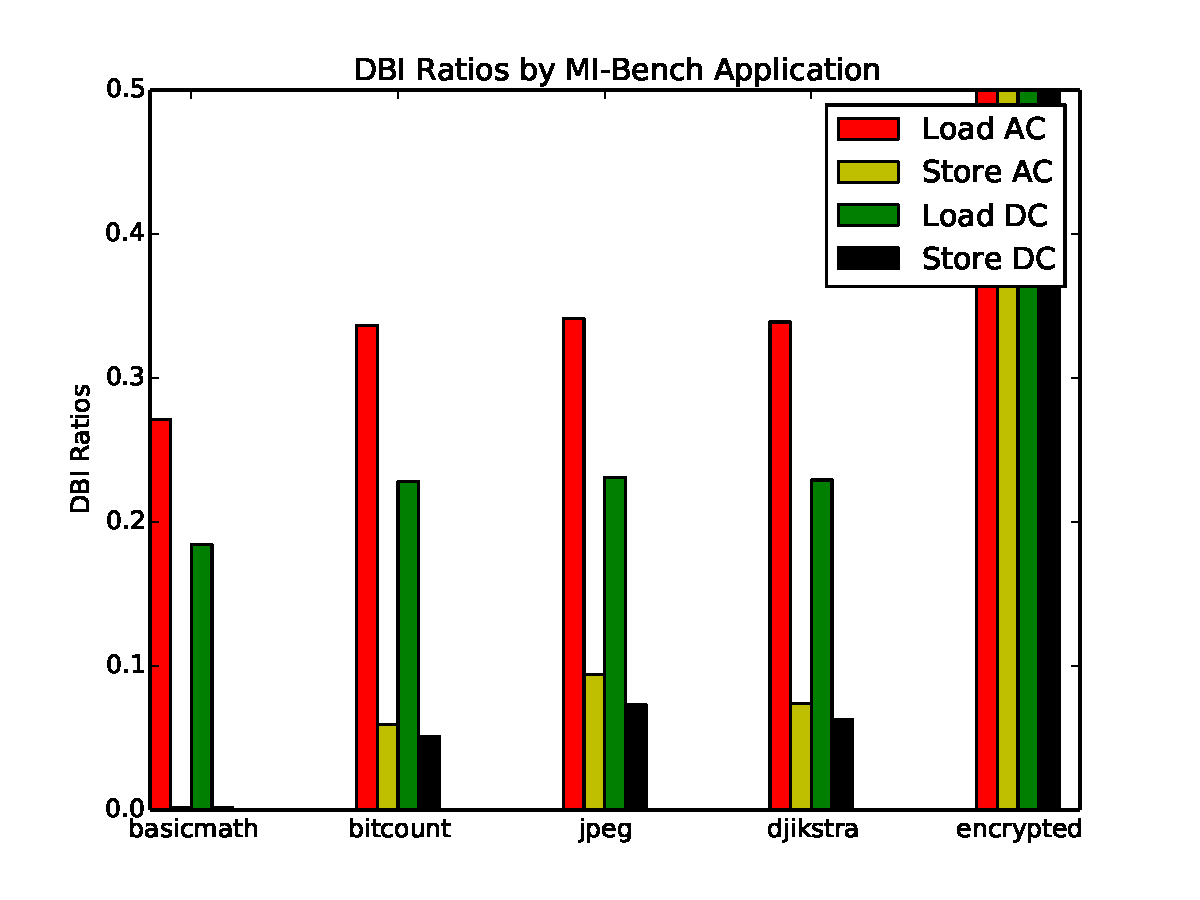
\includegraphics[width=0.5\textwidth]{figs/dbiGraph}
  \caption{Comparing load/store DBI ratios for representative MiBench applications}
  \label{fig:dbiGraph}
\end{figure}

Figure \ref{fig:dbiGraph} illustrates the DBI-AC and DBI-DC ratios for select
MiBench applications and our encrypted system model. The MiBench applications
chosen: \TT{basicmath}, \TT{bitcount}, \TT{jpeg}, and \TT{djikstra} span the
\TT{automotive}, \TT{consumer} and \TT{network} application classes of MiBench.

\begin{enumerate}
  \item Looking at A, B ratios for loads and stores.
  \item Put graphs and analyze them.
  \item Intuition for decrease (store is lower - mostly misses)
\end{enumerate}
